\section{Pr�sentation de l'�tude}
\label{sec:exist}

\subsection{Introduction}
Le cadre de notre �tude consiste en la mise en place d'une infrastructure
permettant la gestion du r�seau d'une organisation r�partie sur plusieurs
sites. Dans notre cas, il s'agit de l'Institut Eur�com, connect� par Internet
� ses Ecoles m�res, l'ENST � Paris et l'EPFL � Lausanne. Et la gestion du
r�seau doit permettre la surveillance de l'�tat op�rationnel de certaines
ressources critiques r�parties sur l'ensemble des trois sites.

\subsection{Existant --- Architecture du r\'eseau}
Le r\'eseau est constitu\'e de trois sites reli\'es par l'Internet. Chacun de
ces sites fonctionne avec:
\begin{htmllist}
  \htmlitemmark{RedBall}
  \item[Cinq serveurs de fichiers SUN]
  \item[Cinq serveurs de calcul HP]
  \item[Un routeur CISCO]
  \item[Trois switchs FORE]
  \item[Un LAN ATM]
\end{htmllist}

De plus, le site d'Eur\'ecom poss\`ede un serveur WEB.\\

\begin{figure}[htbp]
  \centering\includegraphics[width=14cm]{reseau.ps}
  \caption{L'architecture du r\'eseau}
\end{figure}

Nous avons r\'eparti les ressources critiques (les serveurs de fichiers et
de calcul) sur les trois switchs pour \'eviter de se trouver sans aucune
ressource en cas de d\'efaillance d'un de ces derniers. D'autre part, la
charge des diff\'erents liens est
ainsi mieux r\'epartie.\\

Le routeur peut �tre associ\'e \`a un Firewall pour filtrer les acc\`es au
r\'eseau interne depuis l'ext\'erieur. A Eur�com le serveur Web est
directement connect\'e sur le routeur pour que les requ\^etes destin\'ees
\`a ce serveur restent dans la partie du r�seau ouverte au public. Nous
avons install\'e une sonde RMON \`a la sortie du routeur pour effectuer des
mesures et des filtrages sur le trafic sortant et uniquement sur celui-ci.\\

Les ressources sont g�r�es par SNMPv1 qui fonctionne avec de l'IP sur ATM.
Le r\'eseau est administr\'e depuis une machine connect\'ee sur le switch
central pour limiter les flux d'informations li\'es \`a l'administration.
Dans le cas o\`u l'ensemble des ressources est g\'er\'e depuis un seul
site, le site d'administration est \'equip\'e d'une console
d'administration suppl\'ementaire.

